\documentclass{article}
\usepackage[utf8]{inputenc}
\usepackage{latexsym}
\usepackage{url}
\usepackage{hyperref}
\usepackage{graphicx}
\hypersetup{colorlinks=true}
\usepackage{enumitem,amssymb}
\newlist{todolist}{itemize}{4}
\setlist[todolist]{label=$\square$}
\usepackage{txfonts}
\usepackage{clrscode3e}
\usepackage{listings}
\usepackage{xcolor}
\usepackage{tikz}
\usepackage{float}
\usepackage{pgfplots}
\usepackage{enumitem}
\usepackage{amssymb}
\pgfplotsset{width=10cm,compat=1.9}
\usepgfplotslibrary{external}
\usepackage[edges]{forest}
\usepackage{amsmath}
\usepackage{hyperref}
\usepackage{wrapfig}
\usepackage[colorinlistoftodos]{todonotes}

\begin{document}

\title{Moving vehicles \\
\large{Group CEN2.2A, II^{nd} year, 2^{nd} semester, Computers}}
\date{\today}
\author{Fr\u{a}sineanu Claudia Andreea}
\maketitle

\newpage
\section{Problem statement}
Let us assume that $m$ vehicles are located in squares (1, 1) through ($m$, 1) (the bottom row) of an $m \times m$ squared parking. The vehicles must be moved to the top row, but arranged in reverse order; so vehicle $i$ starting from $(i, 1)$ must end up in $(m - i + 1, m)$. On each time step, each of the $m$ vehicles is restricted to move only one square up, down, left, or right, or keep current position (i.e. does not move); but if a vehicle does not move, one other adjacent vehicle (but not more than one) can hop over it. Two vehicles cannot occupy the same square.

\begin{itemize}
    \item[a.] Write a detailed formulation for this search problem.
    \item[b.] Identify a suitable search algorithm for this task and explain your choice.
\end{itemize}

\section{Approach}
First and foremost we need to determine the bounds between which our solution can vary. To find these limits, we will take into consideration the worst and best cases.


First, we take the case where we have a single car in the parking lot. Because it cannot jump over any other cars, then the distance of it, from a point $(i, 1)$ to $(m-i, m)$ would be the same as the \emph{Manhattan distance}. This would give us the upper bound.

The second case will give us the lower bound, and is the ideal scenario, in which a car will be able to jump over all the cars until it reaches its place. Because the car actually moves over two blocks every time, it means that it will reach the destination in half the usual time, thus in \emph{half of the Manhattan distance}.

Now that we have determined the bounds, we can safely assume that an optimal heuristic for our search algorithm would be given by the Manhattan distance.


Since the given problem is a dynamic one, it becomes clear that we will need to keep track of all the cars and decide which ones to move, and into which direction. Thus the algorithm will be divided into two parts: the \emph{states} each car can be in, and a proper \emph{search algorithm} that will take into consideration both the states and our heuristic function.


\subsection{States}
\label{states}
Each of the cars can have one of the following states: \emph{move down}, \emph{move up}, \emph{move right}, \emph{move left}, \emph{jump down}, \emph{jump up}, \emph{jump right}, \emph{jump left}, \emph{remain in the current position}.

The key elements regarding the states are the conditions used to ensure that the cars will not move out of bounds. At each step, we will check the conditions for each move, and, if the action can be completed, then it is added to the list of actions.

\subsection{Heuristic}
As I mentioned above, an optimal heuristic for this problem would be the one given by the \emph{Manhattan distance}. Thus, the function implementing this will be:

\begin{center}
    $h = \sum \vert currentState - goalState \vert * 2$
\end{center}

\subsection{Search function}
\label{search_function}

To ensure that the most optimal algorithm is chosen, we can test for a simple case each of the search algorithms. We will take into consideration three major factors: the \emph{total cost of the path}, because we need to provide one of the most cost efficient solutions, the \emph{total considered actions}, since they have a crucial impact on the overall performance of the algorithm, and the \emph{runtime}. 


An important thing to note is the fact that the way the initial and goal state is organized, greatly affects the performance of the algorithms. There are cases where certain search algorithms are not working because they are returning an \emph{empty} path and thus are not able to call any other functions.

In order to better emphasize these differences, I conducted tests for the two possible layouts. I took into consideration four important search algorithms: \emph{Breadth First Search} on a graph, \emph{Depth First Search} on a graph, \emph{Best First Search} and \emph{A* Search}. For each of these I ran two tests, to see how their performance changes with the size of the parking lot.

Without further due, in the two tables below can be seen the results of the tests conducted if the input and output state looked like this:

\begin{center}
    


\[ InitialState = 
\begin{bmatrix}
1 & 0 & 0 & 0\\
2 & 0 & 0 & 0\\
3 & 0 & 0 & 0\\
4 & 0 & 0 & 0\\
\end{bmatrix}
,\space \space  GoalState =  
\begin{bmatrix}
0 & 0 & 0 & 4\\
0 & 0 & 0 & 3\\
0 & 0 & 0 & 2\\
0 & 0 & 0 & 1\\
\end{bmatrix}
\]
\bigskip

\begin{tabular}{l*{3}{c}r}
Size = 3 & Path Cost & Possible Actions & Runtime\\
\hline
Breadth First   & 11 & 995 & 0.008072   \\
Depth First     & - & - & -   \\
Best First      & 21 & 389 & 0.00715  \\
A*              & 11 & 782 & 0.01463   \\
\end{tabular}

\bigskip

\begin{tabular}{l*{3}{c}r}
Size = 4 & Path Cost & Possible Actions & Runtime\\
\hline
Breadth First   & 17 & 130063 & 56.80981   \\
Depth First     & 161 & 889 & 0.01267   \\
Best First      & 64 & 8407 & 0.41881 \\
A*              & - & - & -   \\
\end{tabular}

\end{center}

\bigskip

We can observe from these that there are significant discrepancies between the behaviours of the search algorithms. On one side, we have \emph{Breadth First Search}, which gives an optimal result, but it takes a lot of time to compile, and on the other side we have \emph{Best First Search}, which gives a non-optimal solution, but within a reasonable runtime. \emph{Depth First Search} and \emph{A*} cannot be taken into consideration because there are cases for which either of them will not work properly.

Now we can proceed to the second layout, where the two states will be :

\begin{center}
    

\[ InitialState = 
\begin{bmatrix}
1 & 2 & 3 & 4\\
0 & 0 & 0 & 0\\
0 & 0 & 0 & 0\\
0 & 0 & 0 & 0\\
\end{bmatrix}
,\space \space  GoalState =  
\begin{bmatrix}
0 & 0 & 0 & 0\\
0 & 0 & 0 & 0\\
0 & 0 & 0 & 0\\
4 & 3 & 2 & 1\\
\end{bmatrix}
\]

\begin{tabular}{l*{3}{c}r}
Size = 3 & Path Cost & Possible Actions & Runtime\\
\hline
Breadth First   & 8 & 246 & 0.00101   \\
Depth First     & - & - & -   \\
Best First      & - & - & -  \\
A*              & 12 & 141 & 0.01213   \\
\end{tabular}

\bigskip

\begin{tabular}{l*{3}{c}r}
Size = 4 & Path Cost & Possible Actions & Runtime\\
\hline
Breadth First   & - & - & -   \\
Depth First     & - & - & -   \\
Best First      & 64 & 8407 & 0.41881 \\
A*              & 19 & 28744 & 16.64201  \\
\end{tabular}

\end{center}

\bigskip

From this data we can gather that there are two search algorithms that have given optimal results: \emph{Breadth First Search}, for the first type of input, and \emph{A* Search}, for the second type of input. But, because \emph{Breadth First Search} takes too much time to compute the results, I will chose to implement \emph{A* Search}, in order to be able to provide more test results.

\subsection{A* Search}
\label{astar_search}

A* is an informed search algorithm, or a best-first search, meaning that it is formulated in terms of weighted graphs: starting from a specific starting node of a graph, it aims to find a path to the given goal node having the smallest cost (least distance travelled, shortest time, etc.). It does this by maintaining a tree of paths originating at the start node and extending those paths one edge at a time until its termination criterion is satisfied.

At each iteration of its main loop, A* needs to determine which of its paths to extend. It does so based on the cost of the path and an estimate of the cost required to extend the path all the way to the goal. Specifically, A* selects the path that minimizes

\begin{center}
    $f(n) = g(n) + h(n)$
\end{center}

where :
\begin{itemize}
    \item $n$ is the next node on the path,
    \item $g(n)$ is the cost of the path from the start node to n,
    \item $h(n)$ is a heuristic function that estimates the cost of the cheapest path from n to the goal.
\end{itemize}

 A* terminates when the path it chooses to extend is a path from start to goal or if there are no paths eligible to be extended. 


\begin{figure}[t]
\begin{center}
\begin{tabbing}
\indent \textbf{fun}\=\textbf{ction} \textsc{A*-Search}($problem, function$) \textbf{returns} a solution node or failure \\

\indent \> $node \leftarrow $ \textsc{Node(State} = \emph{problem.} \textsc{Initial)}\\

\indent \> $frontier \leftarrow $ a priority queue ordered by f, with \emph{node} as an element \\

\indent \> $explored \leftarrow $ a set containing all the visited nodes \\

\indent \> \textbf{if} \emph{problem.} \textsc{goal-test} \emph{(node.} \textsc{state)} \textbf{then return} \emph{node} \\

\indent \> \textbf{while not} \= \textsc{is-empty} \emph{(frontier)} \textbf{do} \\

\indent \> \> $node \leftarrow $ \textsc{pop} \emph{(frontier)} \\

\indent \> \> \textbf{if} \emph{problem.} \textsc{goal-state} \emph{(node.} \textsc{state)} \textbf{then return} \emph{node} \\
 
 \indent \> \> $explored \leftarrow $ \textsc{add} \emph{(node.} \textsc{state)} \\
 
\indent \> \> \textbf{for each} \= \emph{child} \textbf{in} \textsc{expand} \emph{(problem, node)} \textbf{do} \\

\indent \> \> \> \textbf{if} \= \emph{child.} \textsc{state} \textbf{is not in} \emph{explored} \textbf{and} \emph{child} \textbf{is not in} \emph{frontier} \textbf{then} \\

\indent \> \> \> \> \ $frontier \leftarrow $ \textsc{add} \emph{(child)} \\

\indent \> \> \> \textbf{elif} \= \emph{child} \textbf{is in} \emph{frontier} \textbf{then} \\

\indent \> \> \> \> $incumbent \leftarrow $ $frontier[child]$ \\

\indent \> \> \> \> \textbf{if} \= $f(child) < f(incumbent)$ \textbf{then} \\

\indent \> \> \> \> \> \textbf{delete} $frontier[incumbent]$ \\

\indent \> \> \> \> \> \ $frontier \leftarrow $ \textsc{add} \emph{(child)} \\

\end{tabbing}
\caption{Pseudocode for A* Search}
\label{fig_alg_ex}
\end{center}
\end{figure}


\section{Experimental Data}
For this problem, the input consists of only one number: the \emph{size of the parking lot}. There are two major limitations of this number: it has to be \emph{positive}, and the maximum value cannot exceed 7, as the tests take too much time to finish and it becomes impossible to obtain the results.

\begin{center}
    $number = \{ randomNumber | randomNumber \in [1, 7] \}$
\end{center}

The matrices used to describe the initial and goal state will be generated within the class constructor, in accordance with the \emph{number}.

\section{Projection of experimental application}


The following section and figures will give further details concerning the structure and organization of the programs. The most important algorithms are separated into their own module, to facilitate the eventual modifications, and, overall to keep the code clean. There is also a separate module for the random generator and two folders where all the input and output files are kept.

\newpage

\subsection{High level application design}
\begin{wrapfigure}{r}{0.5\textwidth}
\centering
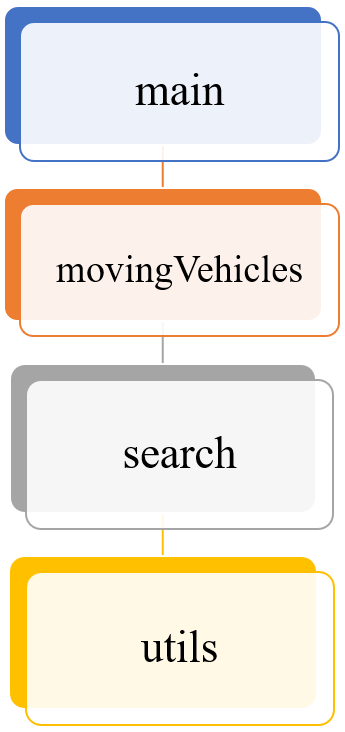
\includegraphics[width=.45\linewidth]{Images/hierarchy.PNG}
\caption{Hierarchy}
\end{wrapfigure}

The hierarchy of the application is fairly simple. At the bottom we have the \emph{utils} module, where are kept some auxiliary functions needed for solving the problem. Above it is the \emph{search} module, inside which lay a few search algorithms, along with the class \emph{Problem}. The module \emph{movingVehicles} contains the actual solution of the problem, with all the data, states and heuristic. At the top we have the \emph{main} module, where the functions are called and where the actual reading, writing and measuring of runtime happens.

The hierarchy of the project folder is shown in the figure below:

\begin{figure}[H]
    \centering
    \begin{forest}
    forked edges,
    for tree = {rectangle, draw, grow=east},
    draw,
    [Project
        [images]
        [Documentation.pdf]
        [Documentation.tex]
        [README.txt] 
        [ OutputData [outputTest6.txt] [...] [outputTest1.txt] ]
        [ InputData [test6.txt] [...] [test1.txt] ]
        [randomGenerator.py ]
        [utils.py ]
        [search.py ]
        [movingVehicles.py ]
        [main.py ]
    ]
    \end{forest}
    \caption{Project hierarchy\\}
    \label{fig:projh}
\end{figure}

\newpage

Below we have a more in-depth description of each folder and module. 
\newline

\begin{enumerate}[label=\Roman*]
  \item \emph{Project\textbackslash InputData}\\
  Contains all the input files needed to generate test cases for the problem.
    \begin{itemize}
        \item \emph{testi.txt}$\rightarrow$ all the tests generated randomly, used to research the time execution and compare the different implementations ; $i=\overline{1,6}$
    \end{itemize}
    
    \item \emph{Project\textbackslash OutputData}\\
    Contains all the output files with the results needed to formulate the conclusions for the problem.
    \begin{itemize}
        \item \emph{outputTesti.txt}$\rightarrow$ the output resulted from each test, with all the necessary data; $i=\overline{1,6}$
    \end{itemize}
    
    \item \emph{Project\textbackslash main.py}\\
   It is the "main" of the python implementation,holding all the calls of the functions necessary for successfully compiling the program.

     \item \emph{Project\textbackslash movingVehicles.py}\\
   Holds the implementation of the problem, extending the class \emph{Problem} and completing its functions.
   
   \item \emph{Project\textbackslash search.py}\\
   Holds the implementation of the problem, extending the class \emph{Problem} and completing its functions. In here we define the states and the heuristic function.
   
   \item \emph{Project\textbackslash utils.py}\\
   Holds the implementation of the problem, extending the class \emph{Problem} and completing its functions. In here we define the states and the heuristic function.
   
\end{enumerate}

\subsection{Implemented functions}
Due to the fact that the structure and hierarchy of the whole project has been taken into consideration, the following subsections will offer further insight regarding each function, variable, as well as the input and output data. 


\begin{enumerate}[label=\Roman*]

\item In \emph{main.py}
    \begin{center}
         \emph{main()} \\
      \end{center}
    Its purpose is to serve as a sort of ”front-end”, dealing only with the initialization of the variables, calls of the functions and measuring the execution time. It also serves as a link both between the subprograms and the input and output files.
    
\item In \emph{movingVehicles.py}
      \begin{center}
          \textbf{class} \emph{MovingVehicles} \emph{(Problem})\\
      \end{center}
     This class is an extension of the class \emph{Problem} found in \emph{search.py} module, and it contains the essential functions needed to solve our search problem and their implementations. 
     
     \begin{enumerate}
%init(self, parkingSize)
    \item \emph{\textunderscore \textunderscore init \textunderscore \textunderscore(\emph{self}, parkingSize)}\\
    This is the constructor of the class, and it takes care of all the variables that need to be initialized. Its only parameter is: 
    \begin{itemize}
        \item $parkingSize \rightarrow$ the size of the parking lot. It is needed in order to create the matrices used to define the initial and goal state. 
    \end{itemize}

%findFirstEmptySpot(self, state)    
    
    \item \emph{findFirstEmptySpot(\emph{self}, state)} \\
    It searches for the next car that can be moved and returns its state. The only variable is:
    \begin{itemize}
        \item $state \rightarrow$ after searching for an empty space, we return the state of the car object at the new position. In order to do that, we need to keep track of all the states. 
    \end{itemize}
         
%actions(self, state)
    \item \emph{actions(\emph{self}, state)} \\
    This is the implementation of the function found in the class \emph{Problem}, in \emph{search.py}. Inside this function are defined all the possible actions a car can make at a given moment. We start with a list of \emph{possible actions}, where we add the "default" action, which is \emph{Stay}. After that we check if we have reached the goal node, and if true, we return the list. 
    
    If we have not reached the goal node, we begin to check if the conditions for each possible move is met, i.e. we ensure that if the car completes the move it does not go outside of bounds. As mentioned in section \ref{states}, all the possible moves an object can make at a time are: \\

    \emph{actions} = \{ Stay, MoveUp, MoveDow, MoveLeft, MoveRight, JumpUp, JumpDown, JumpLeft, JumpRight \} \\

    If the car satisfies the conditions and can move into one of these directions, then the \emph{action} is added to the list of \emph{possible actions}. After going through all possibilities, the variable \emph{self.consideredActions} is increased. This variable serves as to show the user how many lists of actions are taken into consideration, compared with what are the ones that are part of the final answer.
    
    \begin{itemize}
        \item $state \rightarrow$ due to the fact that it is a dynamic problem, we need a way to keep track of all the states of the cars in order to determine their possible actions. Thus, the variable containing these states needs to be updated and passed around.
    \end{itemize}         
         
%result(self, state, action) 
    \item \emph{result(\emph{self}, state, action)} \\
    Like the above function, this is also the implementation of the function with the same name from the class \emph{Problem}. Its main scope is to return the state that results from executing the given action in the given state. Hence, the two parameters are:
    
\begin{itemize}
    \item $state \rightarrow$ contains a list of the states in which the objects can be found.
    \item $action \rightarrow$ the action from which we decide the outcome
\end{itemize}
         
%heuristic(self, node)
    \item \emph{heuristic(\emph{self}, node)} \\
    At each step we compute the heuristic for the given node and return its value.
    \begin{itemize}
        \item $node \rightarrow$ the current node from which we want to determine the heuristic.
    \end{itemize}
     
    \end{enumerate}
%--------End of movingVehicles.py ------------------

\item In \emph{search.py}

\begin{center}
    \textbf{class} \emph{Problem}
\end{center}
      
      This is the abstract class upon which I based the class \emph{MovingVehicles}. It contains all the necessary functions for this problem. The most notable functions, which have not been yet discussed are:
      
      \begin{enumerate}
          \item \emph{goal \textunderscore test(\emph{self}, state)} \\
          This acts as a \emph{bool} function, returning true only if the state is the same as the goal state.
          \begin{itemize}
              \item $state \rightarrow$ the state we want to check
          \end{itemize}
          
         \item \emph{path \textunderscore cost(\emph{self}, c, state1, action, state2 )} \\
          There was no need for me to modify this function, as it returns the proper result. In this particular case, the last three function parameters are not needed.
          \begin{itemize}
              \item $c \rightarrow$ the cost of the path so far.
          \end{itemize}
          
      \end{enumerate}
      
      \begin{center}
          \textbf{class} \emph{Node}
      \end{center}
      
      This class is the structure of a single node inside a graph. A single node is characterized by the following parameters:
      \begin{itemize}
          \item [$\textasteriskcentered$] $state \rightarrow$ the current state of the node
          \item [$\textasteriskcentered$] $parent \rightarrow$ the parent of the current node
          \item [$\textasteriskcentered$] $action \rightarrow$ the action that can be performed by the node
          \item [$\textasteriskcentered$] $path \textunderscore cost \rightarrow$ the total cost of the path
          \item [$\textasteriskcentered$] $depth \rightarrow$ if the current node has a parent, then its depth is equal to the depth of the parent node plus one.
      \end{itemize}
      
      An important thing to node regarding this class is the fact that I have change the way the path is printed.
      
      \begin{enumerate}
          \item \emph{\textunderscore \textunderscore repr  \textunderscore \textunderscore (\emph{self})} \\
          This function returns a printable representational string of the given object. Thus, instead of printing the matrix as a list, it can now be printed as an actual matrix. This was done in order to facilitate the visual parsing of the solution.
          
      \end{enumerate}
      
\item \emph{breadth \textunderscore first \textunderscore graph \textunderscore search(problem)}  \\
This, along with a few more functions, have been left inside the module in case we want to test the problem using different types of search algorithms.

This particular function searches the deepest nodes in the search tree first. Unlike \emph{Breadth First Search} on a tree, this function does not get trapped in loops.
Its performances can be seen in \ref{search_function}. This method brings the most efficient path in terms of cost, but it performs badly in terms of runtime, which is why I did not choose it as my search function.

\item \emph{depth \textunderscore first \textunderscore graph \textunderscore search(problem)}  \\
Just like the algorithm above, this one too, does not get caught in loops. It goes through the deepest nodes in the graph first, and then makes its way upwards. As seen in section \ref{search_function}, this algorithm performed badly on all the cases, so it cannot be used for this problem.

\item \emph{best \textunderscore first \textunderscore graph \textunderscore search(problem, f)}  \\
This function is called by the \emph{A* Search}, the only difference being in the use of functions. Because \emph{A*} uses a more complex system, it yields better results.

\item \emph{astar \textunderscore search(problem, f)}  \\
This is the final search algorithm left in the module, and is also the one I choose for the problem, due to the complexity of its function \emph{f}. Further details regarding both the algorithm and the pseudocode can be found in section \ref{astar_search}.


\end{enumerate}


\subsection{Input data}
To generate our input data we need only one number: the size of the parking lot, \emph{m}. Because we will always now what the initial and goal states will look like, we can generate them inside the class constructor. Thus, the input read from file will be: 

\[ Input = \{ m & \quad | & \quad m=\text{size of the parking lot} \}
\]

\subsection{Output data}
The output is generated by the implemented algorithm, and placed in text file. I first chose to print the matrices corresponding to each step, so we can picture the way the cars are moving in the parking lot. Immediately after that, it will be printed the actions the cars take throughout the algorithm in order to reach their destination. The next two lines will contain the total cost of the path, and the number of all the actions the program considers during runtime. I chose to include this to show how complex the search becomes after just a few increases in the size of the matrix. The last line contains the execution time of the program, which was needed, like the previous variable, to show how the algorithm behaves on different test cases.

The structure of the output will be:

\[ Output =
  \begin{cases}
    ml, & \quad ml=\text{list of matrices}\\
    l, & \quad l=\text{list of actions}\\
    cost, & \quad cost=\text{total cost of the algorithm}\\
    actions, & \quad actions=\text{actions taken into consideration}\\
    time, & \quad t=\text{execution time}
  \end{cases}
\]

It should be noted that the list of matrices can only be printed in the console, because its print function is dependent on the \emph{\textunderscore \textunderscore repr \textunderscore \textunderscore()} function. In order to make it write the data in a file, it would be needed to pass that file as parameter and that would change the functions unnecessarily. 

\section{Results}
As we said before, this is a dynamic problem, meaning we have to take into consideration the state of each of the $m$ cars. Due to its complex nature it is difficult to find an algorithm that will yield both the lowest cost for the path and the most efficient runtime.  The main focus was upon finding a solution that could best approximate the final result, within a reasonable runtime. 

Through trial and error, I have narrowed the best search algorithms to the four major ones: \emph{Breadth First Search}, \emph{Depth First Search}, \emph{Best First Search} and \emph{A* Search}. After running test and analyzing the results that can be found in section \ref{search_function}. Thus, as I mentioned previously, the algorithm capable of offering a middle ground between the two aspects was \emph{A* Search}. It is true that it did not offer the best solutions, and that there is room for improvement. Unfortunately, as will be seen from the graph of the execution time, even for small numbers all the algorithms took a long time to complete and so my choices were limited.

In the image below there is an example of the console output for a case where the parking size is equal to three.

\begin{figure}[htp]
         \centering
             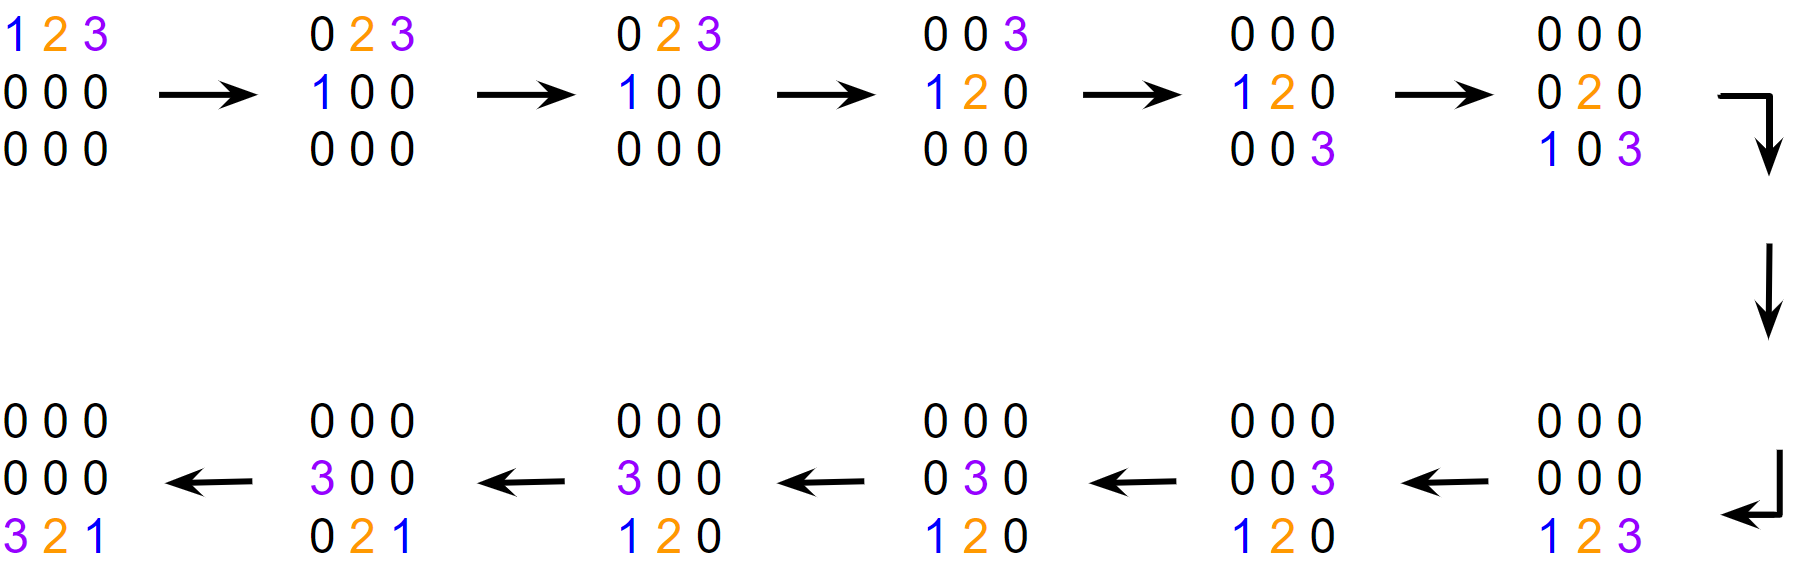
\includegraphics[width=10cm,height=4cm]{Images/exemplu.PNG}
             \caption{Example}
             \label{fig:example}
        \end{figure}

From this example we can deduce that the algorithm is providing a near optimal solution. We can also see they way it takes into consideration all the other solutions and the states of the other cars. In addition to this, the function which determines the total cost of the path is correct and returns the proper value.

The tables below contain the actual data gathered after running test on the algorithm.

\bigskip

\begin{center}
    \begin{tabular}{l*{3}{c}r}
 A* Search &  Path Cost & Possible Actions & Runtime\\
\hline
m = 2   & 6 & 17 & 0.000009543   \\
m = 3   & 11 & 629 & 0.00901937   \\
m = 4   & 19 & 28774 & 16.64201235  \\
m = 5   & 40 & 49635 & 1637.28562839  \\
m = 6   & 76 & 83713 & 3743.27394039   \\
m = 7   & 134 & 150342 & 7438.82732398 \\
\end{tabular}
\end{center}

\bigskip

Using this data the following three graphs have been generated:

\begin{figure}[H]
    \centering
    \begin{multicols}{2}
        \centering
        \begin{tikzpicture}
\begin{axis}[
    axis lines = left,
    ylabel = Path Cost,
    xlabel = Matrix Size,
    legend style={at={(0.37,0.9)},anchor=center},
    width=5cm,
    height=5cm,
    no markers
]
\addplot table[x=Test,y=Time] {path_cost.txt};
\end{axis}
\end{tikzpicture}
        \begin{tikzpicture}
\begin{axis}[
    axis lines = left,
    ylabel = Runtime (seconds),
    xlabel = Matrix Size,
    legend style={at={(0.37,0.9)},anchor=center},
    width=5cm,
    height=5cm,
    no markers
]
\addplot table[x=Test,y=Time] {runtime.txt};
\end{axis}
\end{tikzpicture}
    \end{multicols}
    \caption{Path Cost and Runtime}
\end{figure}

%possible actions
\begin{figure}[H]
    \centering
    \begin{multicols}{2}
        \centering
        \begin{tikzpicture}
\begin{axis}[
    axis lines = left,
    ylabel = Possible Actions,
    xlabel = Matrix Size,
    legend style={at={(0.37,0.9)},anchor=center},
    width=5cm,
    height=5cm,
    no markers
]
\addplot table[x=Test,y=Time] {possible_actions.txt};
\end{axis}
\end{tikzpicture}
\end{multicols}
\end{figure}


\section{Conclusions}
The assignment I was handed proved to be challenging on a few aspects. At first it was a bit difficult to adapt my problem to the material provided in laboratory. After that I had to make sure that I had the right formulas when checking whether a car will be out of the matrix' bounds. 

But the most notable I think was the fact that I could not provide the output for non-trivial numbers. Because the search became so complex due to the many actions it had to take into consideration, the number of test had to be limited to numbers smaller than ten. Yet, there is important information to gather and many conclusions to be taken even if the information is scarce.

All in all, although challenging, I learned a lot, both by researching and implementing different algorithms to see which would suit my problem better. I made significant progress and I am pleased with the fact that I managed to find an almost optimal solution to this problem.




% bibliography
\begin{thebibliography}{9}

	\bibitem{aima2010}
	  Stuart Russell and Peter Norvig,
	  \emph{Artificial Intelligence: A Modern Approach}.
	  Prentice Hall,
	  3rd Edition,
	  2010.

    \bibitem{lamport94}
	 \url{http://theory.stanford.edu/~amitp/GameProgramming/Heuristics.html},
	  \emph{Heuristics},
	   (accessed at May $29^{th}$ 2021).

    \bibitem{lamport94}
	 \url{https://en.wikipedia.org/wiki/A*_search_algorithm},
	  \emph{A* Search},
	   (accessed at May $29^{th}$ 2021).
	   
	   
	\bibitem{lamport94}
	 \url{https://isaaccomputerscience.org/concepts/dsa_search_a_star},
	  \emph{A* Search Algorithm},
	   (accessed at May $30^{th}$ 2021).
	 
	\bibitem{framework}
	  \emph{problem \textunderscore solving \textunderscore framework.zip}, uploaded on Google Classroom \emph{Artificial Intelligence D27CEL427}, on May $5^{th}$ 2021
	  
	\bibitem{tablesOveleaf}
	 \url{https://www.overleaf.com/learn/latex/Tables},
	  \emph{Tables in \LaTeX },
	   (accessed at June $4^{th}$ 2021). 
	   
	\bibitem{graphs}
	 \url{https://www.overleaf.com/learn/latex/TikZ_package},
	  \emph{Graphics in \LaTeX },
	   (accessed at June $4^{th}$ 2021). 
	   
\end{thebibliography}

\end{document}
